\documentclass[11pt,letterpaper,titlepage]{article}



\usepackage[spanish]{babel}
\usepackage{epsfig}
\usepackage{graphicx}
\usepackage{graphics}
\usepackage{xcolor}



\usepackage[colorlinks=false, bookmarks=false, urlcolor=black]{hyperref}

\usepackage[a4paper]{geometry}
\geometry{top=1.0in, bottom=1.0in, left=1in, right=1in}

\newcommand{\grad}{\hspace{-2mm}$\phantom{a}^{\circ}$}
% 
% \usepackage{hyperref}
% \hypersetup{
%     colorlinks,
%     citecolor=black,
%     filecolor=black,
%     linkcolor=black,
%     urlcolor=black
% }

\begin{document}
\begin{titlepage}
\begin{center}
{\large Universidad Auton\'oma Metropolitana}
% \vskip 0.1cm
{\large unidad Azcapotzalco\\}
% \vskip 0.1cm
{\large Divisi\'on de Ciencias B\'asicas e Ingenier\'ia\\}
% \vskip 0.1cm
{\large Ingener\'ia en Computaci\'on\\}
{\large Propuesta de proyecto terminal\\}
\vskip .6cm
{\large{{\it Linkuam, ``Sistema de apoyo para la difusi\'on de ideas innovadoras y emprendedoras''.}}}
%\large{{\it Traductor entre diagramas de flujo y c\'odigo ANSI C, capaz de visualizar y editar ambas representaciones.}}

\vskip 2.6cm
{\large {Jorge Alberto Bautista Hern\'andez}\\}
{\large {201301215}\\}
{\large {Trimestre 10-O, \today{}}}
%\date{} %Investigar que onda con la fecha

\vskip 2.7cm
{\large \flqq{Me comprometo  a asegurar que el alumno cuente con los recursos materiales necesarios para que \'esta propuesta se realice satisfactoriamente.\frqq}\\}
\vskip .3cm
{\large Dra. Ma. Lizbeth Gallardo L\'opez\\}
{\large No. eco. 30761}
\end{center}


\end{titlepage}

\tableofcontents

  \begin{abstract}
% progreso - estancamiento
\textit{Innovar}\footnote{Mudar o alterar algo, introduciendo novedades. \textit{Fuente: \href{http://www.rae.es/}{http://www.rae.es/}}} y \textit{emprender}\footnote{Acometer y comenzar una obra, un negocio, un empe\~no, especialmente si encierran dificultad o peligro.  \textit{Fuente: \href{http://www.rae.es/}{http://www.rae.es/}}} son verbos que en la actualidad marcan la l\'inea divisoria entre un seguidor y un l\'ider. Para que M\'exico pueda progresar y mantener ese progreso durante un largo tiempo, debe convertirse en un l\'ider, innovando y emprendiendo. Partiendo sobre todo de las que deber\'an de ser sus principales generadoras de talento, conocimiento y soluciones a problemas en nuestra sociedad: sus universidades\cite{papeluniversidad}. 

Cambiemos la forma en que vemos a nuestras universidades, pensemos en ellas como centros para la convivencia y preparaci\'on de personas que pueden cambiar el rumbo de nuestro pa\'is y del mundo, y no solo como un lugar donde vienen los j\'ovenes a tomar una educaci\'on superior. Preparemos a los j\'ovenes para que sean capaces de tomar liderazgos en un ambiente como en el que M\'exico se encuentra actualmente inmerso. 

La actividad de promover una cultura emprendedora e innovadora que ayude a este prop\'osito, bien puede apoyarse en un sistema inform\'atico.
  \end{abstract}

\section{Objetivo general}
% [ANTES]
% El objetivo principal de este proyecto terminal es desarrollar una aplicaci\'on web que facilite la difusi\'on y ayude en la gesti\'on de ideas generadas por miembros de la UAM \footnote{Entiendase como ``miembro de la UAM'' o ``comunidad universitaria'' a todo aquel que estudie y trabaje (o lo haya hecho) en cualquiera de los planteles de la UAM.}, promoviendo as\'i una cultura innovadora y emprendedora dentro de nuestra Universidad, que a largo o corto plazo, tengan como efecto mejoras significativas en el nivel de vida de nuestro pa\'is.
% (AHORA)
\textcolor{black}{El principal objetivo de este proyecto terminal es promover una cultura innovadora y emprendedora dentro de nuestra Universidad, a trav\'es del desarrollo de una aplicaci\'on web que facilite la difusi\'on y ayude en la gesti\'on de ideas de proyectos generadas por miembros de la UAM}\footnote{Entiendase como ``miembro de la UAM'' o ``comunidad universitaria'' a todo aquel que estudie y trabaje (o lo haya hecho) en cualquiera de los planteles de la UAM.}.
% , que a largo o corto plazo, tengan como efecto mejoras significativas en el nivel de vida de nuestro pa\'is.



% o ``comunidad de estudiantes'' o ``comunidad estudiantil''

\section{Objetivos particulares}
\textcolor{black}{
\subsection{Registrar las ideas creativas de los miembros de la UAM}
Se desarrollar\'a un m\'odulo que permita a los miembros de nuestra Universidad registrar aquellas ideas que podr\'ian ayudar a la UAM o a nuestra sociedad. }
% Ideas que casi siempre mueren en un olvido provocado por apat\'ia, falta de inter\'es, tiempo, etc.

% \subsection{Facilitar el inicio de ideas  innovadoras y emprendedoras}

\textcolor{black}{
\subsection{Difundir ideas entre la comunidad universitaria}
Se desarrollar\'a un m\'odulo que permita iniciar, publicar, criticar y retroalimentar ideas (por ejemplo para proyectos de vinculaci\'on, para iniciar una empresa, proyectos de investigaci\'on, etc.) propuestas por miembros de la UAM e incluso por egresados de la misma. Esta informaci\'on ser\'a difundida a los miembros de la comunidad universitaria, a trav\'es de una p\'agina Web.}

% \subsection{Difusi\'on de actividades}
% Este proyecto terminal ayudar\'a a difundir informaci\'on sobre las actividades emprendidas entre miembros de nuestra comunidad universitaria.

% \subsection{Surgimiento de l\'ideres}
% Este sistema busca permitir a los miembros emprendedores de una comunidad universitaria una f\'acil iniciaci\'on de actividades, de tal manera que surjan alumnos y profesores l\'ideres dentro de una universidad.

% \subsection{Surgimiento de empresas}
% Facilitando la gesti\'on de actividades interdisciplinarias, se pretende promover la creaci\'on de empresas dentro de una comunidad universitaria.

\subsection{Difundir proyectos en proceso de desarrollo}
\textcolor{black}{
Un m\'odulo que permita la publicaci\'on y difusi\'on de propuestas de proyectos tanto de servicio social como de proyecto terminal; proporcionando as\'i un repositorio de opciones, para los alumnos interesados en cubrir estos requerimientos.}

%\subsection{M\'as opciones para proyecto terminal}
%\textcolor{black}{
%Se desarrollar\'an funcionalidades que faciliten la publicaci\'on y difusi\'on de actividades propuestas (por miembros de la UAM) para realizarse como proyecto terminal, proporcionando m\'as opciones a alumnos y acad\'emicos para elegir este requerimiento.}
% para su titulaci\'on, as\'i como una m\'as adecuada elecci\'on de proyectos por parte del asesor.

%\subsection{Facilitar participaci\'on de estudiantes egresados}\textcolor{black}{
%Un m\'odulo que facilite a miembros egresados, de la Universidad Aut\'onoma Metropolitana, participar en proyectos que se lleven a cabo dentro de la UAM e incluso proponer y/o emprender ideas. }
% Introduciendo as\'i la experiencia en el \'ambito profesional de estos egresados, a proyectos que se lleven a cabo dentro de la UAM.
\textcolor{black}{
\subsection{Facilitar la comunicaci\'on con diferentes comunidades}
Un m\'odulo que facilite a miembros y no miembros de la Universidad, la publicaci\'on de problemas que enfrenta su comunidad o instituci\'on; y que por supuesto buscan apoyo dentro de nuestra comunidad estudiantil y acad\'emica. }
% Esto podr\'ia dar pie a crear una puerta de enlace con la sociedad
% , que es realmente a la que una Universidad debe servir.
% Con este proyecto terminal pretendo desarrollar una aplicaci\'on web que facilite el inicio y difusi\'on de actividades innovadoras dentro de una universidad, promoviendo as\'i un esp\'iritu emprendedor entre los estudiantes y logrando el surgimiento de l\'ideres universitarios.

% \subsection{Eliminar el miedo a crear cosas nuevas}
% Para que este proyecto terminal rinda frutos es necesario implantar medidas que ayuden a nuestra comunidad universitaria a olvidar miedos que cohiben la creaci\'on de propuestas de valor.

\section{Antecedentes}
\subsection{Referencias internas}
% Luego de buscar y revisar proyectos terminales realizados por parte de los alumnos de Ingenier\'ia en Computaci\'on de la Universidad Aut\'onoma Metropolitana, no hemos encontrado ninguno con objetivos similares a los que planteamos en este proyecto.\footnote{A pesar de que existen proyectos terminales a los que bien podr\'ia hacerse referencia en esta secci\'on debido a la afinidad de los temas que tratan, no existe informaci\'on alguna sobre sus reportes finales en la p\'agina de la Divisi\'on de Ciencias B\'asicas e Ingenier\'ia ni en la zona correspondiente de la biblioteca.}

\begin{itemize}

  \item \textcolor{black}{\textit{\textbf{Sistema basado en web para la gesti\'on de capital intelectual referente a la organizaci\'on de las metodolog\'ias de las TIC.}}}

\textcolor{black}{Este sistema es una aplicaci\'on web que permite la difusi\'on y publicaci\'on de informaci\'on relacionada con tecnolog\'ias inform\'aticas, as\'i como la posibilidad de publicar, descargar y vender cursos a trav\'es de \'el.}

\textcolor{black}{Nuestro proyecto terminal tambi\'en tiene como objetivo difundir informaci\'on, sin embargo, no ser\'a exclusiva de tecnolog\'ias TI. Tampoco planteamos ning\'un objetivo donde se requieran funcionalidades para poder comerciar informaci\'on.}

  \item \textcolor{black}{\textit{\textbf{Sistema de administraci\'on de proyectos terminales.}}}

\textcolor{black}{Sistema que permite gestionar la informaci\'on de los proyectos terminales que se han desarrollado hasta el momento en la UAM-A. Tambi\'en permite llevar un control de los asesores y estudiantes relacionados con determinado proyecto.}

\textcolor{black}{Nuestro proyecto terminal propone difundir proyectos terminales a realizarse; no as\'i un histor\'ico sobre los ya realizados.}

  \item \textcolor{black}{\textit{\textbf{Sistema de gesti\'on de informaci\'on de programas de responsabilidad social.}}}

\textcolor{black}{Este sistema tiene como objetivo gestionar las actividades de responsabilidad social, para poder medir sus alcances y resultados en el futuro.}

\textcolor{black}{Nuestro proyecto terminal tambi\'en hace \'enfasis en el registro de actividades; sin embargo, no tiene como objetivo medir los alcances de las actividades que se registrar\'an y difundir\'an en \'el.}

\end{itemize}


\subsection{Referencias externas}
\begin{itemize}
% \item \textit{\textbf{Red mexicana de emprendedores - \'Angeles inversionistas y emprendedores-  \'Angel Ventures M\'exico}}
\item \textit{\textbf{Red mexicana de emprendedores $\&$  \'Angel Ventures M\'exico}}

El objetivo principal de estas asociaciones es servir de enlace entre proyectos innovadores y personas que pueden invertir monetariamente en \'estos. Adem\'as clasifican las diferentes propuestas e inversiones haciendo a\'un m\'as sencilla su vinculaci\'on.

\textcolor{black}{Red mexicana de emprendedores plantea una idea: ``Existen proyectos que necesitan capital y existen capitales que pueden ser invertidos; nosotros los vincularemos.''. }


\textcolor{black}{Al igual que ``Red mexicana de emprendedores'', uno de los fines que tiene este proyecto terminal, es comunicar a miembros de la UAM que generen ideas con otros miembros que puedan ejecutarlas, aunque estas ideas no sean necesariamente empresas.}

\textit{\textbf{Direcci\'on en internet:}}\href{http://www.angelesinversionistas.com.mx}{http://www.angelesinversionistas.com.mx}\\
\textit{\textbf{Direcci\'on en internet:}}\href{http://www.angelventuresmexico.com}{http://www.angelventuresmexico.com}


\item \textit{\textbf{Emprendimiento, Tecnol\'ogico de Monterrey}}

Con el objetivo de continuar promoviendo y desarrollando el esp\'iritu emprendedor en sus alumnos, el Tecnol\'ogico de Monterrey ha creado el Instituto para el Desarrollo de Emprendedores, a travé\'es del cual se les brindan las herramientas necesarias para crear, iniciar, consolidar y hacer crecer sus propias empresas. 

\textcolor{black}{El Tecnol\'ogico de Monterrey cuenta con muchas herramientas disponibles para alumnos emprendedores, desde asesor\'ia en el inicio de sus proyectos, pasando por b\'usqueda de capital e incluso apoyo en cuestiones de patentes.}

\textcolor{black}{Nuestro proyecto terminal podr\'ia, en un futuro, servir de catapulta en cada una de las fases de los proyectos que alumnos emprendedores lleven a cabo, tal como lo hace el Tecnol\'ogico de Monterrey.}

\textit{\textbf{Direcci\'on en internet:}}\href{http://www.itesm.edu/wps/wcm/connect/ITESM/Tecnologico+de+Monterrey/Emprendimiento/#2}{http://www.itesm.edu}



\end{itemize}


\section{Justificaci\'on}
\subsection{Innovar y emprender}
Innovar y emprender han llevado a muchos pa\'ises a convertirse en los l\'ideres del mundo en la actualidad y est\'an llevando a otros a convertirse en los l\'ideres del futuro. Sin enfocarnos solo a la cuesti\'on del progreso monetario, los pa\'ises m\'as innovadores y emprendedores est\'an generando soluciones para muchos de los problemas que afectan al mundo.

Lamentablemente, M\'exico no cuenta con una cultura innovadora ni emprendedora de calidad en sus universidades (p\'ublicas). Como resultado, la mayor\'ia de nuestros alumnos no innovan o emprenden a lo largo de su estancia en la Universidad, se limitan a hacer lo que sus tareas les exigen. Esto no quiere decir que nuestros alumnos no sean capaces de innovar o emprender (!`todo lo contrario!), es simplemente una falta de atenci\'on por parte de acad\'emicos y autoridades de la Universidad hacia cuatro cosas: espacios donde la comunidad universitaria pueda publicar, criticar, iniciar y desarrollar ideas; espacios para promover una amplia comunicaci\'on entre nuestra comunidad universitaria (alumnos, acad\'emicos y autoridades universitarias de diferentes carreras y divisiones, incluso planteles); difusi\'on de planes de apoyo que la UAM ofrece para el inicio y desarrollo de ideas emprendedoras; y tal vez la m\'as importante de todas: hacer conscientes a todos los miembros de la UAM de que realmente pueden orientar sus esfuerzos a innovar, a emprender, y no necesariamente a seguir esquemas ya impuestos por la industria actual\cite{desarrollo}.

\subsection{Innovar y emprender en la UAM}

Durante el periodo de tiempo que he estado estudiando en la UAM Azcapotzalco, he tenido muy pocos profesores que aborden, en su clase, sobre las actividades que podemos (?`tal vez ``debemos''?, desde el punto de vista de apoyar a nuestra sociedad) realizar cuando terminemos nuestros estudios, o incluso durante el transcurso de estos. Y de estos pocos acad\'emicos que lo hacen, la gran mayor\'ia de ellos han impuesto a su clase una manera de pensar muy particular. Entre las ideas que imponen esa manera de pensar se citan las siguientes:
\begin{itemize}
 \item \flqq{Preparense para trabajar en empresas que existen ``all\'a afuera''.}\frqq
 \item \flqq{La competencia ``all\'a afuera'' est\'a muy fuerte.} \frqq
 \item \flqq{Los planes de estudio de su carrera no sirven ``all\'a afuera''.}\frqq
\item \flqq{Esto es solo una pr\'actica, realmente aprender\'an ``all\'a afuera''.}\frqq
%  \item etc.
\end{itemize}
 

Pasando por alto las ``muchas quejas'' y ``pocas soluciones'', jam\'as nos mencionan que hay otra opci\'on diferente al ``all\'a afuera'', jam\'as nos mencionan que tambi\'en existe la opci\'on de comenzar una empresa y/o actividad remunerada propia, que no es forzoso que los estudiantes universitarios trabajemos para una empresa ya existente (teniendo que adaptarnos a su sistema), sino que !`podemos ser los creadores de nuestra propia empresa! y que de hecho, nuestro pa\'is necesita m\'as que nunca de estudiantes creadores de empresas con ideas innovadoras que impulsen nuestra econom\'ia y propongan soluciones a muchos problemas en los que M\'exico est\'a inmerso. No quiero decir que trabajar en una empresa ya establecida sea malo, lo que intento transmitir es que muchas veces se limita nuestra visi\'on del mundo laboral, omitiendo comentarios que nos hacen saber que tambi\'en podemos innovar y emprender. No solamente acad\'emicos y autoridades de nuestra Universidad promueven y terminan fijando esta manera de pensar en nuestros estudiantes, hay otros factores por ejemplo: la pobre comunicaci\'on existente entre los alumnos de las diferentes divisiones de la UAM Azcapotzalco, e incluso de diferentes carreras:

Supongamos que uno de nuestros dise\~nadores industriales quisiera deleitar con sus creaciones al mundo, y emprender un negocio comenzando con una galer\'ia en alg\'un lugar de Polanco, probablemente necesitar\'ia de un par de dise\~nadores gr\'aficos para crear una p\'agina web atractiva y la imagen de su local; un ingeniero en computaci\'on que desarrolle su sistema de pagos en l\'inea; un contador para no tener problemas con la SHCP; un abogado para cuestiones legales e ingenieros en computaci\'on, mec\'anica y electr\'onica que le ayuden a impactar al p\'ublico creando estantes m\'oviles rob\'oticos donde nuestro dise\~nador pueda mostrar sus obras. Los alumnos de universidades p\'ublicas no cuentan con recursos monetarios suficientes para poder producir estas ideas, nuestro dise\~nador tendr\'ia que preocuparse por algo m\'as que la belleza y originalidad de sus obras. La inversi\'on para la realizaci\'on de esta idea, no es despreciable, considerando que debe pagar honorarios. Si la inversi\'on pudiera dedicarse exclusivamente a la apertura del negocio, ahorrando en recursos humanos, esto facilitar\'ia la ejecuci\'on de su idea. Consideramos que nuestro dise\~nador puede recurrir a su Universidad, en ella puede encontrar a otros estudiantes emprendedores\cite{emprendedurismo} para poder comenzar su negocio: dise\~nadores, ingenieros, abogados, etc. Incluso podr\'ia encontrar asesor\'ia para poder atraer inversiones y as\'i pagar los sueldos de profesionistas. !`Es cuesti\'on de comunicaci\'on!...He ah\'i el problema, en la UAM Azcapotzalco no existe la suficiente comunicaci\'on \-entre los alumnos incluso ni entre acad\'emicos, ni entre las autoridades de las diferentes Divisiones y/o carreras\-, como para que proliferen este tipo de actividades; actividades que beneficiar\'ian tanto a los participantes en el negocio, como al prestigio de nuestra Universidad.

Si nuestro alumno quisiera buscar dentro de la UAM estos recursos, ?`c\'omo los encontrar\'ia?, probablemente hay personas emprendedoras que quisieran participar en proyectos de este tipo, pero ?`c\'omo se enterar\'ian de la existencia de este proyecto? Claro que se puede recurrir a pegar folletos en todas las paredes de la UAM, pero la contaminariamos visualmente como lo hacemos (de forma lamentable) en tiempos de votaciones o de huelgas, sobretodo si cada alumno con una idea se decidiera a pegar sus propios papelitos.

En este proyecto planteamos una forma de iniciar y dar difusi\'on a actividades emprendedoras e innovadoras dejando limpia nuestra UAM y manteniendo informados sobre ellas tanto a alumnos como a acad\'emicos y autoridades.

\subsection{Servicio social}

Para poder egresar de la UAM Azcapotzalco necesitamos cumplir con 480 horas de servicio social. Estas horas pueden realizarse tanto en instituciones de gobierno como en PyMES\footnote{Empresa mercantil, industrial, etc., compuesta por un n\'umero reducido de trabajadores, y con un moderado volumen de facturaci\'on. \textit{Fuente: \href{http://www.rae.es/}{http://www.rae.es/}}}.

Se supone que esta actividad ``social'' debe de beneficiar a la sociedad, sin embargo, muchos de los proyectos en los que nuestros estudiantes deciden realizar su servicio, se alejan mucho de este cometido social. Esto deriva en que nuestros estudiantes son explotados por las instituciones donde realizan su servicio, con pretextos como ``experiencia'' o ``contrataciones futuras''. Este tipo de consecuencias puede deberse a dos razones: la apat\'ia del estudiante por escoger un servicio social adecuado o la falta de variedad en actividades aceptadas que pueden realizarse como servicio social.

Actualmente, para elegir que actividad realizar\'an como servicio, nuestros estudiantes pueden elegir de una carpeta de proyectos o pueden ir a un instituci\'on y ``escoger'' entre un conjunto de actividades ya determinadas  (si tienen suerte).  ?`Qu\'e pasar\'ia si nuestros estudiantes pudieran proponer la actividad que quieren realizar como servicio social? Te\'oricamente deber\'ian de proponer actividades mucho m\'as \'utiles a la sociedad, en las que se sentir\'ian muy c\'omodos trabajando. Suponiendo que esto \'ultimo fuera verdad, no ser\'ia sencillo para un alumno encontrar a quien pudiera hacer v\'alidas estas horas de servicio.
%  (no se trata solo de que los dise\~nadores practiquen bocetaje o que los abogados aprendan a litigar ?`o s\'i?)


Imaginemos que a un emprendedor estudiante de sociolog\'ia se le ocurre la idea de realizar, junto con otros compa\~neros de dise\~no gr\'afico e industrial, un libro con las fotograf\'ias m\'as representativas de la UAM, recopilando im\'agenes de sus lugares y momentos m\'as bellos a trav\'es del tiempo, recorriendo sus diferentes planteles. Este libro se le regalar\'ia a cada alumno de la Universidad, teniendo como objetivo aumentar el sentido de identidad en nuestra comunidad estudiantil (que buena falta nos hace). Esta idea interdisciplinaria es buena (a mi parecer), ?`pero a qui\'en le es \'util? ?`qui\'en querr\'ia (y podr\'ia hacer v\'alidas) 480 horas dedicadas a esa actividad interdisciplinaria?...nos encontramos con el mismo problema: mala (incluso inexistente) comunicaci\'on entre alumnos, acad\'emicos y autoridades de la Universidad.

En este proyecto planteamos una forma de proponer actividades para servicio social por parte de la comunidad universitaria, ampliando el abanico de proyectos aceptados, promoviendo as\'i que las actividades realizadas realmente ayuden a la sociedad. Estas nuevas actividades propuestas, ser\'an difundidas a estudiantes y acad\'emicos, logrando as\'i que alguien interesado en ellas, pueda hacerlas v\'alidas.


\subsection{Proyecto terminal}
Otro requisito para poder egresar de la carrera de Ingenier\'ia en Computaci\'on, es la realizaci\'on de un proyecto terminal, para lo cual requerimos al menos de un asesor que nos gu\'ie a lo largo del desarrollo de este proyecto.

Lo que nosotros los alumnos hacemos normalmente, es buscar a nuestro asesor, vamos de cub\'iculo en cub\'iculo preguntando por la lista de proyectos terminales de cada profesor y buscamos uno que se nos resulte interesante. En el mejor de los casos, tambi\'en proponemos un nuevo proyecto terminal al profesor, que con algo de suerte nos aceptar\'a. Aqu\'i suceden dos cosas. Primero, si el profesor nos ofrece su lista de proyectos y nosotros tomamos uno, estamos dejando de proponer nuestras ideas para la realizaci\'on de nuestro proyecto. ?`Por qu\'e no emprender ideas innovadoras con nuestro proyecto terminal? Segundo, si nosotros proponemos un nuevo proyecto terminal a un profesor y este nos lo acepta, ?`estamos seguros de que ese asesor es el adecuado para guiarnos?, tal vez exista un profesor en la UAM de otra carrera o divisi\'on, con m\'as experiencia en los temas relacionados con el proyecto, que permita maximizar los frutos y la utilizaci\'on de \'este.

Habiendo mencionado dos principales formas en que nuestros alumnos definen sus proyectos terminales y a sus asesores, nos parece pertinente proponer al menos 2 opciones m\'as.

Como tercer alternativa a las formas de elecci\'on de proyecto terminal, los profesores podr\'ian elegir a sus asesorados, es decir, los alumnos podr\'ian proponer sus proyectos terminales (tomandose la libertad de emprender e innovar) y los profesores podr\'ian proponerse como asesores de los proyectos terminales que se lleven mejor con su experiencia y/o temas de investigaci\'on. Esto, podr\'ia no solo maximizar los frutos de un proyecto terminal, haciendolo \'util en uno o varios Departamentos de la UAM, en otras universidades o a la sociedad en general. Incluso podr\'ia aumentar el n\'umero de art\'iculos de investigaci\'on que la UAM publica\footnote{Este \'ultimo fen\'omeno es posible ya que un profesor investigador puede encontrar, entre proyectos terminales propuestos por la comunidad universitaria, uno que funcione perfectamente a los fines de sus investigaciones.}.

Como cuarta alternativa, los profesores podr\'ian publicar y difundir entre la comunidad estudiantil los proyectos terminales que a ellos les parecen interesantes o que ser\'ian de ayuda para sus investigaciones.

En este proyecto planteamos una forma de ayudar a los alumnos a proponer sus propios proyectos terminales y que los profesores m\'as adecuados para guiarlos, puedan proponerse como asesores. De la misma manera, planteamos una manera de que los profesores puedan difundir, entre la comunidad de estudiantes, las ideas que ellos tienen para realizar un proyecto terminal y que los estudiantes puedan escogerlo.

\subsection{Aprovechamiento de conocimiento generado}
Existe un sentido de identidad muy d\'ebil en la mayor\'ia de los alumnos de la UAM comparado con el de instituciones como el IPN y la UNAM. Esto se debe principalmente a la forma en que funciona nuestra Universidad: los alumnos pueden ``escoger''\footnote{Usamos esta palabra entre comillas porque deda la falta de recursos y la mala planeaci\'on de los horarios de clase por parte de las autoridades de la Universidad, es casi imposible que la mayor\'ia de nuestros alumnos queden satisfechos con la elecci\'on de sus horarios.}  su horario de clases para poder adaptarlo a sus necesidades laborales o familiares, lo que provoca que en cada trimestre tengan compa\~neros nuevos, haciendo muy dificil el surgimiento de lazos fraternales fuertes entre estudiantes de nuestra Universidad.

Como un efecto secundario, esa escasez de sentido de identidad y de lazos fraternales, provoca que nuestros egresados no participen en actividades dentro de la Universidad posteriores a su titulaci\'on, ocasionando que la Universidad no tenga una retroalimentaci\'on de todo ese conocimiento y experiencia proporcionados a sus alumnos.

Si la UAM pudiera promover una constante comunicaci\'on con sus egresados una vez que estos ya han terminado sus estudios superiores, ellos podr\'ian apoyar, entre otras cosas, a mejorar la calidad de nuestros proyectos terminales, a fortalecer los conocimientos con los que terminan nuestros nuevos egresados, a proporcionar ideas que pudiesen mejorar el estado de nuestra Universidad, ideas para servicio social, ideas para proyectos terminales, podr\'ian proporcionarnos constantes fuentes de empleo para nuevos egresados, podr\'ian incluso ser asesores de proyectos terminales gracias a la experiencia que han adquirido, entre otras muchas ventajas.

En este proyecto planteamos una forma de mantener una comunicaci\'on constante con los egresados de la Universidad Aut\'onoma Metropilitana y sobre todo hacerlos participes en nuevas actividades posteriores a su titulaci\'on, aprovechando sus nuevos conocimientos y experiencias.

\subsection{Compromiso con la sociedad}
Los miembros de la Universidad Aut\'onoma Metropolitana, as\'i como todas las universidades p\'ublicas de nuestro pa\'is, tenemos un compromiso con nuestra sociedad: proponer soluciones a los problemas en los que M\'exico se encuentra inmerso y emprender nuevas ideas que hagan de nuestro pa\'is un l\'ider en el mundo, mejorando el nivel de vida en todo nuestro territorio.

Muchos problemas presentes en nuestra sociedad pueden ser y est\'an siendo resueltos por nuestra unversidad, pero hay muchos otros problemas de los que ni siquiera estamos enterados.
Si la sociedad tuviera una forma de comunicar sus problemas a la UAM, nuestras comunidades acad\'emicas y estudiantiles podr\'ian resolverlos. La resoluci\'on de estos problemas dejar\'ian beneficios tanto a la sociedad como a la misma UAM:
\begin{itemize}
 \item Nos dejar\'ian conocimiento y experiencia derivados de la investigaci\'on realizada para resoverlos.
 \item Nos dar\'ian prescencia en m\'as lugares del pa\'is, lo que aumentar\'ia el prestigio de nuestra Universidad a nivel nacional, incluso internacional\cite{ingenioi}. 
 \item Muchos de esos problemas podr\'ian ser orientados para realizarse como proyectos terminales o servicio social, lo que le dar\'ia mucho m\'as sentido al esfuerzo de nuestros acad\'emicos y estudiantes.
\end{itemize}

Este proyecto plantea una forma para crear un enlace de comunicaci\'on entre nuestra sociedad y nuestra Universidad, pudiendo as\'i trabajar en conjunto para resolver problemas que al final, a todos nos afectan.

%%%%Aqui voy acabo de pegar lo que Jorge agregó en la versión 3 de su documento

% 
% \subsection{Creaci\'on de empresas}
% Hemos comentado a lo largo de esta secci\'on lo importante que es promover en los alumnos una cultura innovadora y emprendedora. Si logramos este objetivo, podemos hacer que la 
% 
% 
% 
% \subsection{?`Qu\'e piensa resolver?}
% 
\section{Descripci\'on t\'ecnica}

Este sistema est\'a pensado para trabajar como una p\'agina web. Funcionar\'a para registrar ideas surgidas en una comunidad universitaria, ayudar a consolidarlas y darles seguimiento. Este seguimiento no ser\'a exhaustivo, este sistema enfocar\'a su atenci\'on  en facilitar el inicio  y consolidaci\'on de las actividades, apoyando tambi\'en en el registro de los eventos y avances m\'as significativos que ocurran mientras dure la ejecuci\'on de la idea.

Son cuatro los tipos de usuario que pueden utilizar el sistema:
\begin{enumerate}
 \item \textbf{Administrador}\\Tiene acceso a todas las funcionalidades del sistema. Tambi\'en se encarga de definir las categor\'ias que diferencian los diferentes tipos de ideas o proyectos.
 \item \textbf{Participante}\\Es un usuario registrado en el sistema y que adem\'as  es participante en alg\'un proyecto o idea.
 \item \textbf{Usuario normal}\\Es un usuario registrado que no tiene participaci\'on en ning\'un proyecto.
 \item \textbf{Usuario no registrado}\\Es un usuario que no se ha registrado en el sistema.
\end{enumerate}


% Las ideas que registradas en el sistema pueden ser usadas como servicio social, proyectos terminales, actividades sociales, seg\'un decida el creador.


% \newpage
\subsection{Casos de uso}


A continuaci\'on se presenta el diagrama de los principales casos de uso de este proyecto terminal.
\begin{center}
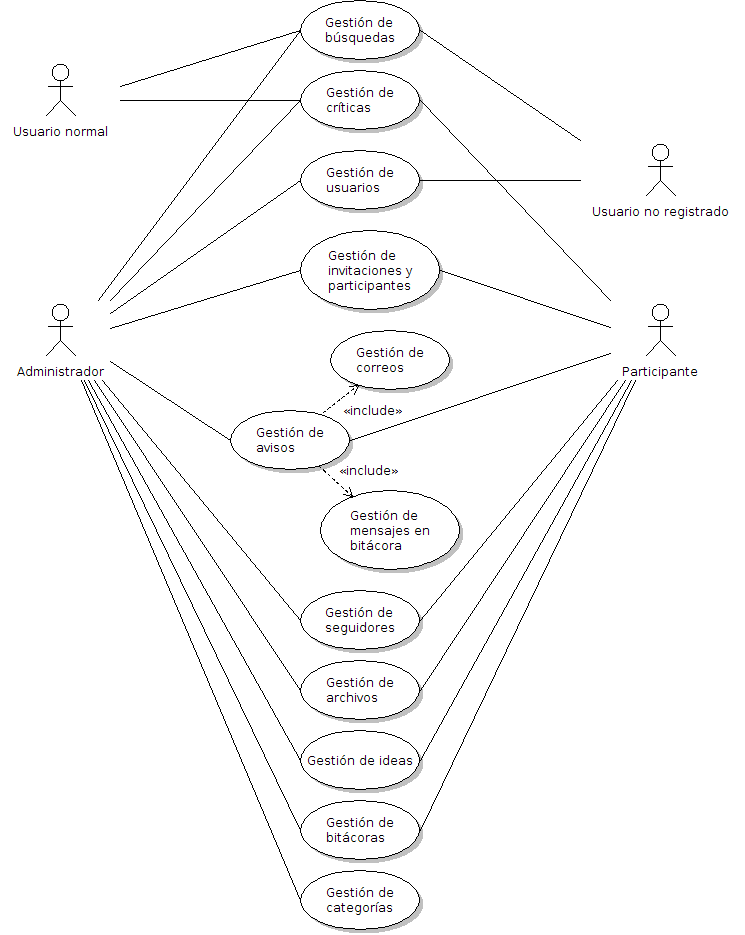
\includegraphics[width=380pt]{casos1.png}
% \caption{Diagrama de casos de uso}
\end{center}


% \subsection{Caracter\'isticas comunes en todas las ideas}
% 
% A continuaci\'on listar\'e la lista de elementos pre
% 
% \begin{itemize}
%  \item  \textbf{Nombre}\\Se refiere al nombre del proyecto.
% 
%  \item  \textbf{Objetivos}\\Se refiere a los objetivos que planea alcanzar la realizaci\'on de esta actividad.
%  \item  \textbf{Justificaci\'on}\\Se refiere a las razones por la que esta actividad planea realizarse.
%  \item  \textbf{Desarrollo de la idea}\\Se refiere a una explicaci\'on m\'as extensa de la idea que pueda ser le\'ida por otros usuarios del sistema.
%  \item  \textbf{L\'ider}\\Se refiere al usuario o usuarios del sistema que tomar\'an el liderazgo del proyecto.
%  \item  \textbf{Participantes}\\Se refiere a las personas que ser\'an participes de esta actividad.
% 
%  \item  \textbf{Invitados a participar}\\Se refiere a los usuarios del sistema que fueron invitados a participar en la actividad, independientemente de que hayan aceptado la invitaci\'on o no.
%  \item  \textbf{Seguidores de la actividad}\\Se refiere a los usuarios del sistema que siguen el progreso de un a actividad a trav\'es de eventos generados en la bit\'acora de los cuales ser\'an avisados.
% 
% \item  \textbf{Bit\'acora de eventos}\\Se refiere al conjunto de eventos y avisos registrados en el sistema por miembros del equipo del proyecto.
% 
% \item \textbf{Cr\'iticas, consejos, preguntas}\\Se refiere al conjunto de preguntas, cr\'iticas y consejos hechos a los miembros de trabajo del equipo por usuarios del sistema, sean miembros o no del proyecto.
% 
% \end{itemize}
% 
% Los elementos mencionados anteriormente ser\'an comunes en todo tipo de ideas, es decir: servicios sociales, proyectos terminales, actividades sociales u otras. Sin embargo, cada una de ellas tendr\'a particularidades propias.

% MANDAR LA ARQUITECTURA A LA ESPECIFICACION TECNICA!!!!!!!!!!!!!!!!!!!!!!!!!!!! 


% \newpage

A continuaci\'on se definen los m\'odulos del sistema:
% La siguiente imagen describe los m\'odulos del sistema: 
% \begin{figure}[htb]
\begin{center} 
%\includegraphics[height=5.3in]{imagenes/Plan2.png}
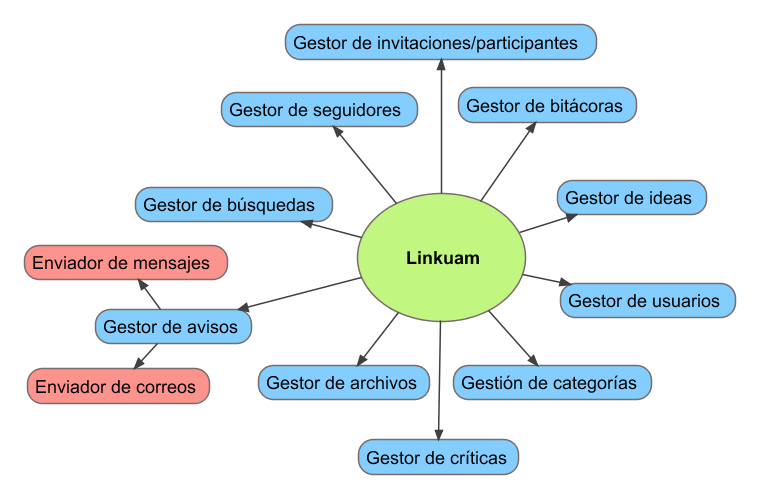
\includegraphics[width=300pt]{arq1.png}
% \caption{Plan de trabajo.}
\end{center}
% \end{figure}

\begin{itemize}

\item \textbf{Gestor de ideas}\\
Este m\'odulo ser\'a el encargado de gestionar las ideas, se encargar\'a del registro, modificaci\'on y eliminaci\'on de estas. Aqu\'i tambi\'en se definir\'a el tipo de idea del que se trata o para que fines funcionar\'a (si es para servicio social, proyecto terminal u otras actividades de apoyo social).

 \item \textbf{Gestor de bit\'acoras}\\
Este m\'odulo ser\'a el encargado de gestionar la bit\'acora del proyecto. Los eventos, avances y avisos importantes ser\'an registrados por miembros del equipo para describir como se ha desarrollado el proyecto a lo largo del tiempo.

 \item \textbf{Gestor de seguidores}\\
Este m\'odulo ser\'a el encargado de administrar los seguidores de un proyecto. Si existen usuarios interesados en determinado proyecto y desean observar su evoluci\'on a lo largo del tiempo, podr\'an suscribirse a este, recibiendo as\'i la informaci\'on que se registre en bit\'acora.

 \item \textbf{Gestor de invitaciones/participantes}\\
Este m\'odulo ser\'a el que permitir\'a invitar a otros usuarios del sistema a participar en la ejecuci\'on de nuevas ideas, difundiendo as\'i la existencia de esta idea entre los miembros de la comunidad estudiantil y acad\'emica. Es en este m\'odulo donde acad\'emicos podr\'ian invitar a los alumnos a participar en sus proyectos y visceversa, as\'i como invitar a alumnos a participar en nuevas actividades como servicio social.


%  \item \textbf{Gestor de ideas}\\
% Este m\'odulo ser\'a el encargado de gestionar la informaci\'on general de las ideas, como el nombre, objetivos, justificaci\'on, desarrollo de la idea y palabras clave.

 \item \textbf{Gestor de usuarios}\\
Este m\'odulo ser\'a el encargado de gestionar a los usuarios del sistema: agregar, editar y eliminar usuarios. El registro de usuarios no se limitar\'a a miembros de la Universidad, sino que podr\'ia abrirse para poder recibir ideas y/o comuncaci\'on de problemas desde otras comunidades externas a la nuestra.

 \item \textbf{Gestor de categor\'ias}\\
Este m\'odulo ser\'a el que permitir\'a definir las categor\'ias a las que puede pertenecer una idea.


 \item \textbf{Gestor de cr\'iticas}\\
Si un usuario quisiera expresar sus dudas, sobre cierto proyecto o quisiera dar una cr\'itica o consejo hacia \'este, el m\'odulo gestor de cr\'iticas ser\'a el encargado de apoyarlo en esta tarea.

 \item \textbf{Gestor de archivos}\\
Puede darse el caso en que sea necesario registrar un archivo, ya sea imagen, texto, binarios, para describir alg\'un evento y/o avance en la ejecuci\'on de la idea. Este m\'odulo ser\'a el que permitir\'a realizar dicha tarea.

 \item \textbf{Gestor de b\'usquedas}\\
Este m\'odulo ser\'a el que permita realizar b\'usquedas de ideas registradas en el sistema. Esta funcionalidad la podr\'an utilizar tanto usuarios registrados como no registrados.

 \item \textbf{Gestor de avisos}\\
Este m\'odulo ser\'a el que permitir\'a manejar todo lo referente a env\'ios de mensajes hacia dentro y hacia fuera del sistema. 
 
\begin{itemize}
 \item  \textbf{Gestor de mensajes}\\
Este m\'odulo ser\'a el que permitir\'a al m\'odulo gestor de bit\'acora registrar mensajes de un proyecto.

 \item \textbf{Gestor de correos}\\
Este m\'odulo ser\'a el que permitir\'a invitar a otros usuarios del sistema a participar en la ejecuci\'on de nuevas ideas a trav\'es de correo electr\'onico y apoyar\'a al m\'odulo gestor de bit\'acora para avisar a los integrantes de un proyecto de que algo ha acontecido.
\end{itemize}
\end{itemize}


\section{Especificaci\'on t\'ecnica}

\textcolor{black}{El siguiente diagrama muestra los bloques principales que compondr\'an al sistema una vez que se encuentre en ejecuci\'on:}

% \textcolor{black}{La siguiente imagen describe la arquitectura del sistema:}
% \begin{figure}[htb]
\begin{center} 
%\includegraphics[height=5.3in]{imagenes/Plan2.png}
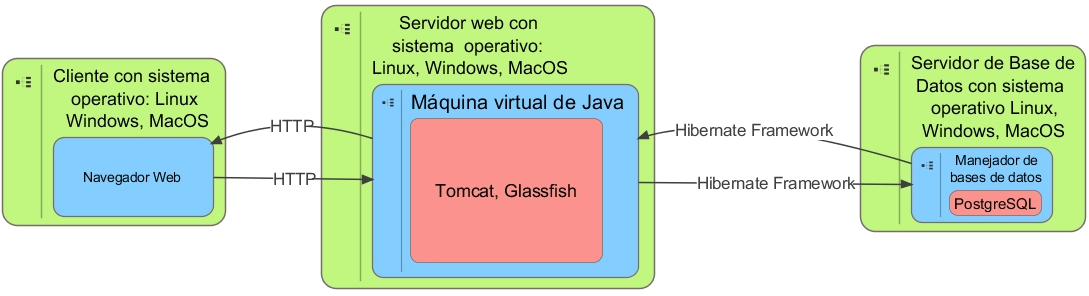
\includegraphics[width=440pt]{arq2.png}
% \caption{Plan de trabajo.}
\end{center}
% \end{figure}
\textcolor{black}{La estructura del sistema cuando se encuentre en ejecuci\'on puede abstraerse a 3 bloques:}

\begin{itemize}
  \item \textcolor{black}{\textbf{Cliente}}

\textcolor{black}{Este bloque se refiere a la computadora del usuario. Las tecnolog\'ias en las que nuestro proyecto terminal ser\'a desarrollado no obligan al usuario a usar un sistema operativo o navegador de internet determinados. Si el usuario cuenta con un navegador web que satisfaga, en su mayor\'ia, los est\'andares de la W3C\footnote{``El Consorcio World Wide Web (W3C) es una comunidad internacional donde las organizaciones Miembro, personal a tiempo completo y el p\'ublico en general trabajan conjuntamente para desarrollar est\'andares Web.'' \href{http://www.w3.org/}{http://www.w3.org/}}, como \textit{Internet Explorer, Firefox, Safari, Konqueror, Chrome}, podr\'a utilizar este sistema. Este bloque se comunicar\'a con el bloque ``Servidor web'' a trav\'es del protocolo HTTP.}

  \item \textcolor{black}{\textbf{Servidor web}}

\textcolor{black}{Este bloque se refiere a la computadora que atender\'a las peticiones que el usuario haga desde el navegador web. Esta computadora deber\'a contar con un servidor de aplicaciones hechas en Java\footnote{\href{http://www.oracle.com/global/lad/technologies/Java/index.html}{http://www.oracle.com/global/lad/technologies/Java/index.html}}  (Tomcat o Glassfish), para lo cual tambi\'en es necesario contar con una m\'aquina virtual de Java instalada. Las tecnolog\'ias en las que nuestro proyecto terminal ser\'a desarrollado obligan a instalar un sistema operativo capaz de ejecutar una m\'aquina virtual de Java.  La comunicaci\'on de este bloque se har\'a tanto con el ``Cliente''(a trav\'es del protocolo HTTP) como con el ``Servidor de base de datos''(utilizando librerias de Hibernate y el protocolo HTTP).}

  \item \textcolor{black}{\textbf{Servidor de base de datos}}

\textcolor{black}{Este bloque se refiere a la computadora que atender\'a las consultas hechas a base de datos por parte del sistema. Las tecnolog\'ias en las que nuestro proyecto terminal ser\'a desarrollado no obligan a usar un sistema operativo determinado, basta con que el manejador de bases de datos utilizado pueda instalarse en \'el. Se utilizar\'a PostgreSQL como manejador de bases de datos. La comunicaci\'on se realizar\'a con el bloque ``Servidor web'' a trav\'es de las librer\'ias de Hibernate y el protocolo HTTP. }

\end{itemize}




\subsection{Alcance del proyecto}

El principal objetivo de este sistema es la gesti\'on de ideas innovadoras surgidas dentro de una comunidad universitaria. Sin embargo, la gesti\'on de estas ideas no se realizar\'a de forma exhaustiva, sino que se enfocar\'a a ayudar a que su ejecuci\'on comience lo m\'as r\'apido posible, proporcionando medios para difundir esta informaci\'on entre la comunidad estudiantil y acad\'emica. 

\textcolor{black}{Para que este sistema se de por concluido, deber\'a ser capaz de proporcionar las siguientes funcionalidades:}

\begin{itemize}
 \item \textcolor{black}{Registrar ideas de proyectos por parte de los miembros y no miembros de la UAM.}
 \item \textcolor{black}{Permitir a quienes proponen proyectos, publicar noticias o mensajes dirigidos a las personas interesadas en esos proyectos.}
 \item \textcolor{black}{Permitir a miembros de la UAM suscribirse a proyectos registrados en el sistema para mantenerse al tanto de eventos que ocurran en marco de ellos.}
 \item \textcolor{black}{Permitir invitar a otros miembros de la UAM (registrados en el sistema) a participar en alg\'un proyecto.}
 \item \textcolor{black}{Permitir a miembros de la comunidad (registrados en el sistema) comentar y criticar las propuestas de los proyectos registrados en el sistema.}
 \item \textcolor{black}{Permitir a miembros de la comunidad realizar b\'usquedas de propuestas de proyectos de su inter\'es.}

\end{itemize}
\textcolor{black}{
\subsection{Licencia}
El software que resulte de este proyecto se pondr\'a a disposici\'on del publico bajo una licencia de software libre \textit{Creative Commons}, espec\'ificamente la licencia tipo: ``Atribuci\'on-No Comercial-Licenciamiento Rec\'iproco 2.5 M\'exico''. Esta licencia declara que se puede copiar, distribuir y comunicar p\'ublicamente la obra, as\'i como hacer obras derivadas, siempre y cuando:}

\begin{itemize}
 \item \textcolor{black}{Se reconozca la autor\'ia de la obra en los t\'erminos especificados por el propio autor o licenciante.}
 \item \textcolor{black}{No utilizar esta obra ni sus derivados para fines comerciales.}
 \item \textcolor{black}{Si se altera, transforma o crea una obra a partir de esta obra, solo se podr\'a distribuir la obra resultante bajo una licencia igual a \'esta.}
\end{itemize}

\textcolor{black}{Una descripci\'on m\'as a detalle de esta licencia se encuentra en esta liga: \\\href{http://creativecommons.org/licenses/by-nc-sa/2.5/mx/}{http://creativecommons.org/licenses/by-nc-sa/2.5/mx/}}
 

% http://creativecommons.org/licenses/by-nc-sa/2.5/mx/


\subsection{Tecnolog\'ias usadas}
Este sistema ser\'a desarrollado como una aplicaci\'on web, siguiendo el modelo cliente-servidor\footnote{\href{http://www.fismat.umich.mx/~anta/tesis/node32.html}{http://www.fismat.umich.mx/~anta/tesis/node32.html}}. En la parte que corresponde al cliente utilizaremos las siguientes tecnolog\'ias:


\begin{itemize}
 \item \textit{HTML}
 \item \textit{Javascript}
 \item \textit{jQuery}
\end{itemize}
En la parte del servidor se har\'a uso de:
\begin{itemize}
 \item \textit{JSP}\footnote{\href{http://java.sun.com/products/jsp/}{http://java.sun.com/products/jsp/}}

 \item Lenguaje de programaci\'on \textit{Java}.
 \item \textit{Java Server Faces}\footnote{\href{http://www.oracle.com/technetwork/java/javaee/javaserverfaces-139869.html}{http://www.oracle.com/technetwork/java/javaee/javaserverfaces-139869.html}}
%  \item Framework \textit{Spring}\footnote{\href{http://www.springsource.org/}{http://www.springsource.org/}}.
 \item \textit{PostgreSQL}\footnote{\href{http://www.postgresql.org/}{http://www.postgresql.org/}}
\end{itemize}


\section{Entregables}

 El reporte final contendr\'a, adem\'as del reporte impreso:
\begin{itemize}
 \item Manual de uso del sistema
 \item Manual de del sistema para desarrolladores
\item C\'odigo fuente del sistema.
 
\end{itemize}





% 
% \section{Glosario[TRABAJANDO]}
% ``miembro de la UAM'' o ``comunidad universitaria'' a todo aquel que estudie y trabaje (o lo haya hecho) en cualquiera de los planteles de la UAM.
% 
% Social Emprending Innoving
% o ``comunidad de estudiantes'' o ``comunidad estudiantil''



 

\section{Calendario de trabajo}
Este proyecto se desarrollar\'a durante el transcurso del trimestre \textit{11-I}.

El trabajo se distribuir\'a en las once semanas de la siguiente manera:

% \begin{center}
% \begin{tabular}{|c|c|}\hline
% Nombre del m\'odulo & Rango de semanas\\ \hline\hline
% %5 & 6 \\ \hline
% Gestor de ideas&1\grad semana \\ \hline
% Gestor de bit\'acoras&2\grad semana \\ \hline
% Gestor de seguidores&2\grad y 3\grad semana\\ \hline
% Gestor de invitaciones/participantes&3\grad y 4\grad semana \\ \hline
% Gestor de b\'usquedas&4\grad semana \\ \hline
% Gestor de usuarios&4\grad y 5\grad semana \\ \hline
% Gestor de categor\'ias&5\grad semana \\ \hline
% Gestor de cr\'iticas&5\grad y 6\grad semana \\ \hline
% Gestor de archivos&7\grad semana\\ \hline
% Gestor de avisos&7\grad y 8\grad semana\\ \hline
% Gestor de mensajes&8\grad y 9\grad semana\\ \hline
% Gestor de correos&9\grad y 10\grad \\ \hline
% Realizaci\'on del reporte final&10\grad y 11\grad \\ \hline
% %6 & 0 \\ \hline
% \end{tabular}
% \end{center}

\begin{center}
\begin{tabular}{|c|c|}\hline
Nombre del m\'odulo & Rango de semanas\\ \hline\hline
%5 & 6 \\ \hline
Gestor de ideas&1\grad semana \\ \hline
Gestor de bit\'acoras&2\grad semana \\ \hline
Gestor de seguidores&2\grad y 3\grad semana\\ \hline
Gestor de invitaciones/participantes&3\grad y 4\grad semana \\ \hline
Gestor de b\'usquedas&4\grad semana \\ \hline
\end{tabular}
\end{center}
\begin{center}
\begin{tabular}{|c|c|}\hline
Gestor de usuarios&4\grad y 5\grad semana \\ \hline
Gestor de categor\'ias&5\grad semana \\ \hline
Gestor de cr\'iticas&5\grad y 6\grad semana \\ \hline
Gestor de archivos&7\grad semana\\ \hline
Gestor de avisos&7\grad y 8\grad semana\\ \hline
Gestor de mensajes&8\grad y 9\grad semana\\ \hline
Gestor de correos&9\grad y 10\grad \\ \hline
Realizaci\'on del reporte final&10\grad y 11\grad \\ \hline
%6 & 0 \\ \hline
\end{tabular}
\end{center}


\textcolor{black}{
\section{Recursos}
\subsection{Financiamiento}
El proyecto terminal no requiere de financiamiento.
\subsection{Recursos disponibles}
Para el desarrollo de este proyecto se cuenta con:}
\begin{itemize}
 \item \textcolor{black}{Una computadora}
  \begin{itemize}
   \item \textcolor{black}{Procesador AMD 64 X2  a 1.8 GHZ }
   \item \textcolor{black}{1GB de RAM}
   \item \textcolor{black}{Sistema operativo Debian\footnote{\href{http://www.debian.org/}{http://www.debian.org/}}.}
   \item \textcolor{black}{Disco duro de 120 GB.}
  \end{itemize}

\end{itemize}

% \begin{itemize}
%  \item Gestor de ideas:
%  \item Gestor de bit\'acoras:
%  \item Gestor de seguidores:
%  \item Gestor de invitaciones/participantes.
%  \item Gestor de ideas:
%  \item Gestor de usuarios:
%  \item Gestor de categor\'ias:
%  \item Gestor de cr\'iticas:
%  \item Gestor de archivos:
%  \item Gestor de avisos:
% 
% \begin{itemize}
%  \item  Gestor de mensajes:
%  \item Gestor de correos:
% \end{itemize}
% 
% \end{itemize}

% \section{Bibliograf\'ia}
% \begin{enumerate}
% 
% % \item University of Georgia. “Points of Pride” University of Georgia,
% %         http://www.uga.edu/profile/pride.html.
% 
% 
%  \item[\textcolor{blue}{[ 1 ]}] \textcolor{black}{Pilar P\'erez Hern\'andez, Rub\'en Oliver Espinoza, Humberto Merritt Tapia, Alejandro M\'arquez, Jorge Le\'on Acevedo, ``\textbf{\textit{El emprendedor en M\'exico: ingenio vs innovaci\'on}}'' \href{http://www.oei.es/memoriasctsi/mesa12/m12p25.pdf}{http://www.oei.es} }
% 
% 
% %  \item \textbf{\textit{El emprendedor en M\'exico: ingenio vs innovaci\'on}}\\
% % \textbf{Autor (es)}:Pilar P\'erez Hern\'andez, Rub\'en Oliver Espinoza, Humberto Merritt Tapia, Alejandro M\'arquez, Jorge Le\'on Acevedo\\
% % \textbf{Direcci\'on en internet}:  \href{http://www.oei.es/memoriasctsi/mesa12/m12p25.pdf}{http://www.oei.es}  \\
% % \textbf{M\'as informaci\'on}: Documento producto del  Congreso Americano de Ciencia, Tecnolog\'ia, Sociedad e Innovaci\'on
% 
% \item[\textcolor{blue}{[ 2 ]}] \textcolor{black}{Instituto Tecnol\'ogico Aut\'onomo de M\'exico (ITAM), ``\textbf{\textit{El papel de las universidades}}'' \href{http://biblioteca.itam.mx/estudios/estudio/letras39-40/texto10/sec\_2.html}{http://biblioteca.itam.mx} }
% 
% % \item \textbf{\textit{El papel de las universidades}}\\
% % \textbf{Autor (es)}:Instituto Tecnológico Autónomo de México (ITAM)\\
% % \textbf{Direcci\'on en internet}:  \href{http://biblioteca.itam.mx/estudios/estudio/letras39-40/texto10/sec\_2.html}{http://biblioteca.itam.mx}\\
% % \textbf{M\'as informaci\'on}: Parte de ``ESTUDIOS. filosofía-historia-letras
% % Invierno 1994 Primavera 1995''
% 
% \item[\textcolor{blue}{[ 3 ]}] \textcolor{black}{Corporaci\'on de estudios para latinoam\'erica(CIEPLAN), ``\textbf{\textit{Innovaci\'on y cultura emprendedora, ?`NECESITAMOS UNA TERCERA V\'IA?}}'' \href{http://www.cieplan.org/archivos/Capitulo\%20046.PDF}{http://www.cieplan.org} }
% 
% 
% % \item \textbf{\textit{Innovaci\'on y cultura emprendedora, ?`NECESITAMOS UNA TERCERA V\'IA?}}\\
% % \textbf{Autor (es)}:Corporaci\'on de estudios para latinoam\'erica(CIEPLAN)\\
% % \textbf{Direcci\'on en internet}:  \href{http://www.cieplan.org/archivos/Capitulo\%20046.PDF}{http://www.cieplan.org}
% 
% \item[\textcolor{blue}{[ 4 ]}] \textcolor{black}{Jairo Edgardo Arias Dur\'an(Programa de Emprendimiento Universidad Industrial de Santander), \textbf{\textit{Resumen del art\'iculo ``Desarrollo de la Cultura Emprendedora}}'' \\\href{http://www.emplenet.org.co/roce/documentos/desarrollo\%20de\%20la\%20cultura\%20emprendedora.pdf}{http://www.emplenet.org.co}}
% 
% % 
% % \item \textbf{\textit{Resumen del art\'iculo ``Desarrollo de la Cultura Emprendedora''}}\\
% % \textbf{Autor (es)}: Jairo Edgardo Arias Dur\'an, ``Programa de Emprendimiento Universidad Industrial de Santander''\\
% % \textbf{Direcci\'on en internet}:  
% %  \href{http://www.emplenet.org.co/roce/documentos/desarrollo\%20de\%20la\%20cultura\%20emprendedora.pdf}{http://www.emplenet.org.co}
% 
% \item[\textcolor{blue}{[ 5 ]}] \textcolor{black}{Annelissie Arr\'azola M., ``\textbf{\textit{EMPRENDEDURISMO}}'' \href{http://produccionintelectual.nur.edu/archivos/emprendedurismo.pdf}{http://produccionintelectual.nur.edu}}
% 
% \item[\textcolor{blue}{[ 6 ]}] \textcolor{black}{Real Academia Espa\~nola, ``\textbf{\textit{Real Academia Espa\~nola}}'' \href{http://www.rae.es}{http://www.rae.es}}

% \section{Bibliograf\'ia}
% \begin{enumerate}
% 
% 
%  \item[\textcolor{blue}{[ 1 ]}] \textcolor{black}{Pilar P\'erez Hern\'andez, Rub\'en Oliver Espinoza, Humberto Merritt Tapia, Alejandro M\'arquez, Jorge Le\'on Acevedo, ``\textbf{\textit{El emprendedor en M\'exico: ingenio vs innovaci\'on}}'' \href{http://www.oei.es/memoriasctsi/mesa12/m12p25.pdf}{http://www.oei.es} }
% 
% \item[\textcolor{blue}{[ 2 ]}] \textcolor{black}{Instituto Tecnol\'ogico Aut\'onomo de M\'exico (ITAM), ``\textbf{\textit{El papel de las universidades}}'' \href{http://biblioteca.itam.mx/estudios/estudio/letras39-40/texto10/sec\_2.html}{http://biblioteca.itam.mx} }
% 
% \item[\textcolor{blue}{[ 3 ]}] \textcolor{black}{Corporaci\'on de estudios para latinoam\'erica(CIEPLAN), ``\textbf{\textit{Innovaci\'on y cultura emprendedora, ?`NECESITAMOS UNA TERCERA V\'IA?}}'' \href{http://www.cieplan.org/archivos/Capitulo\%20046.PDF}{http://www.cieplan.org} }
% 
% \item[\textcolor{blue}{[ 4 ]}] \textcolor{black}{Jairo Edgardo Arias Dur\'an(Programa de Emprendimiento Universidad Industrial de Santander), \textbf{\textit{Resumen del art\'iculo ``Desarrollo de la Cultura Emprendedora}}'' \\\href{http://www.emplenet.org.co/roce/documentos/desarrollo\%20de\%20la\%20cultura\%20emprendedora.pdf}{http://www.emplenet.org.co}}
% 
% \item[\textcolor{blue}{[ 5 ]}] \textcolor{black}{Annelissie Arr\'azola M., ``\textbf{\textit{EMPRENDEDURISMO}}'' \href{http://produccionintelectual.nur.edu/archivos/emprendedurismo.pdf}{http://produccionintelectual.nur.edu}}
% 
% \item[\textcolor{blue}{[ 6 ]}] \textcolor{black}{Real Academia Espa\~nola, ``\textbf{\textit{Real Academia Espa\~nola}}'' \href{http://www.rae.es}{http://www.rae.es}}
% 
% 
% \end{enumerate}

\begin{thebibliography}{99}
\bibitem{papeluniversidad} \textcolor{black}{Instituto Tecnol\'ogico Aut\'onomo de M\'exico (ITAM), ``\textbf{\textit{El papel de las universidades}}'' \href{http://biblioteca.itam.mx/estudios/estudio/letras39-40/texto10/sec\_2.html}{http://biblioteca.itam.mx} } 
\bibitem{desarrollo} \textcolor{black}{Jairo Edgardo Arias Dur\'an(Programa de Emprendimiento Universidad Industrial de Santander), \textbf{\textit{Resumen del art\'iculo ``Desarrollo de la Cultura Emprendedora}}'' \\\href{http://www.emplenet.org.co/roce/documentos/desarrollo\%20de\%20la\%20cultura\%20emprendedora.pdf}{http://www.emplenet.org.co}}
\bibitem{emprendedurismo} \textcolor{black}{Annelissie Arr\'azola M., ``\textbf{\textit{EMPRENDEDURISMO}}'' \href{http://produccionintelectual.nur.edu/archivos/emprendedurismo.pdf}{http://produccionintelectual.nur.edu}}
\bibitem{ingenioi} \textcolor{black}{Pilar P\'erez Hern\'andez, Rub\'en Oliver Espinoza, Humberto Merritt Tapia, Alejandro M\'arquez, Jorge Le\'on Acevedo, ``\textbf{\textit{El emprendedor en M\'exico: ingenio vs innovaci\'on}}'' \href{http://www.oei.es/memoriasctsi/mesa12/m12p25.pdf}{http://www.oei.es} }
% \bibitem{tercervia} \textcolor{black}{Corporaci\'on de estudios para latinoam\'erica(CIEPLAN), ``\textbf{\textit{Innovaci\'on y cultura emprendedora, ?`NECESITAMOS UNA TERCERA V\'IA?}}'' \href{http://www.cieplan.org/archivos/Capitulo\%20046.PDF}{http://www.cieplan.org} }


\bibitem{rae} \textcolor{black}{Real Academia Espa\~nola, ``\textbf{\textit{Real Academia Espa\~nola}}'' \href{http://www.rae.es}{http://www.rae.es}}

% \bibitem{TACWeb} TAC Web-Seite: \url{http://www.tac-global.com}
% \bibitem{PHP} PHP Web-Seite: \url{http://www.php.net}
\end{thebibliography}

\end{document}
